\newpage
\section{Конструкторская часть}

Рассмотрим алгоритмы поиска подстроки в строке.

\subsection{Функциональная модель}

На рисунке \ref{img:idef0} представлена функциональная модель IDEF0
первого уровня.

\begin{figure}[H]
    \centering
    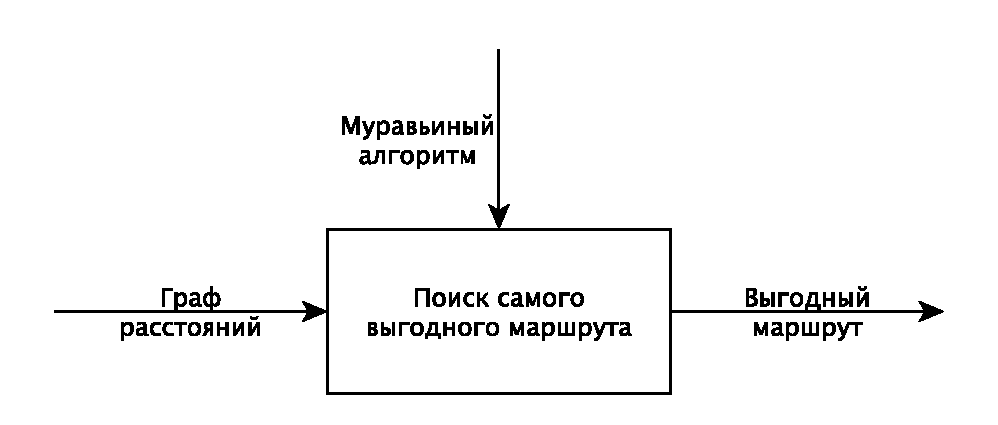
\includegraphics[scale=0.9]{idef0}
    \caption{IDEF0 первого уговня}
    \label{img:idef0}
\end{figure}

\subsection{Схемы алгоритмов}

На рисунках \ref{img:kmp} и \ref{img:bm} представлены схемы алгоритмов.
На рисунке \ref{img:fail} представлена схема создания массива сдвигов
для алгоримта Кнута-Морриса-Пратта.

\begin{figure}[H]
    \centering
    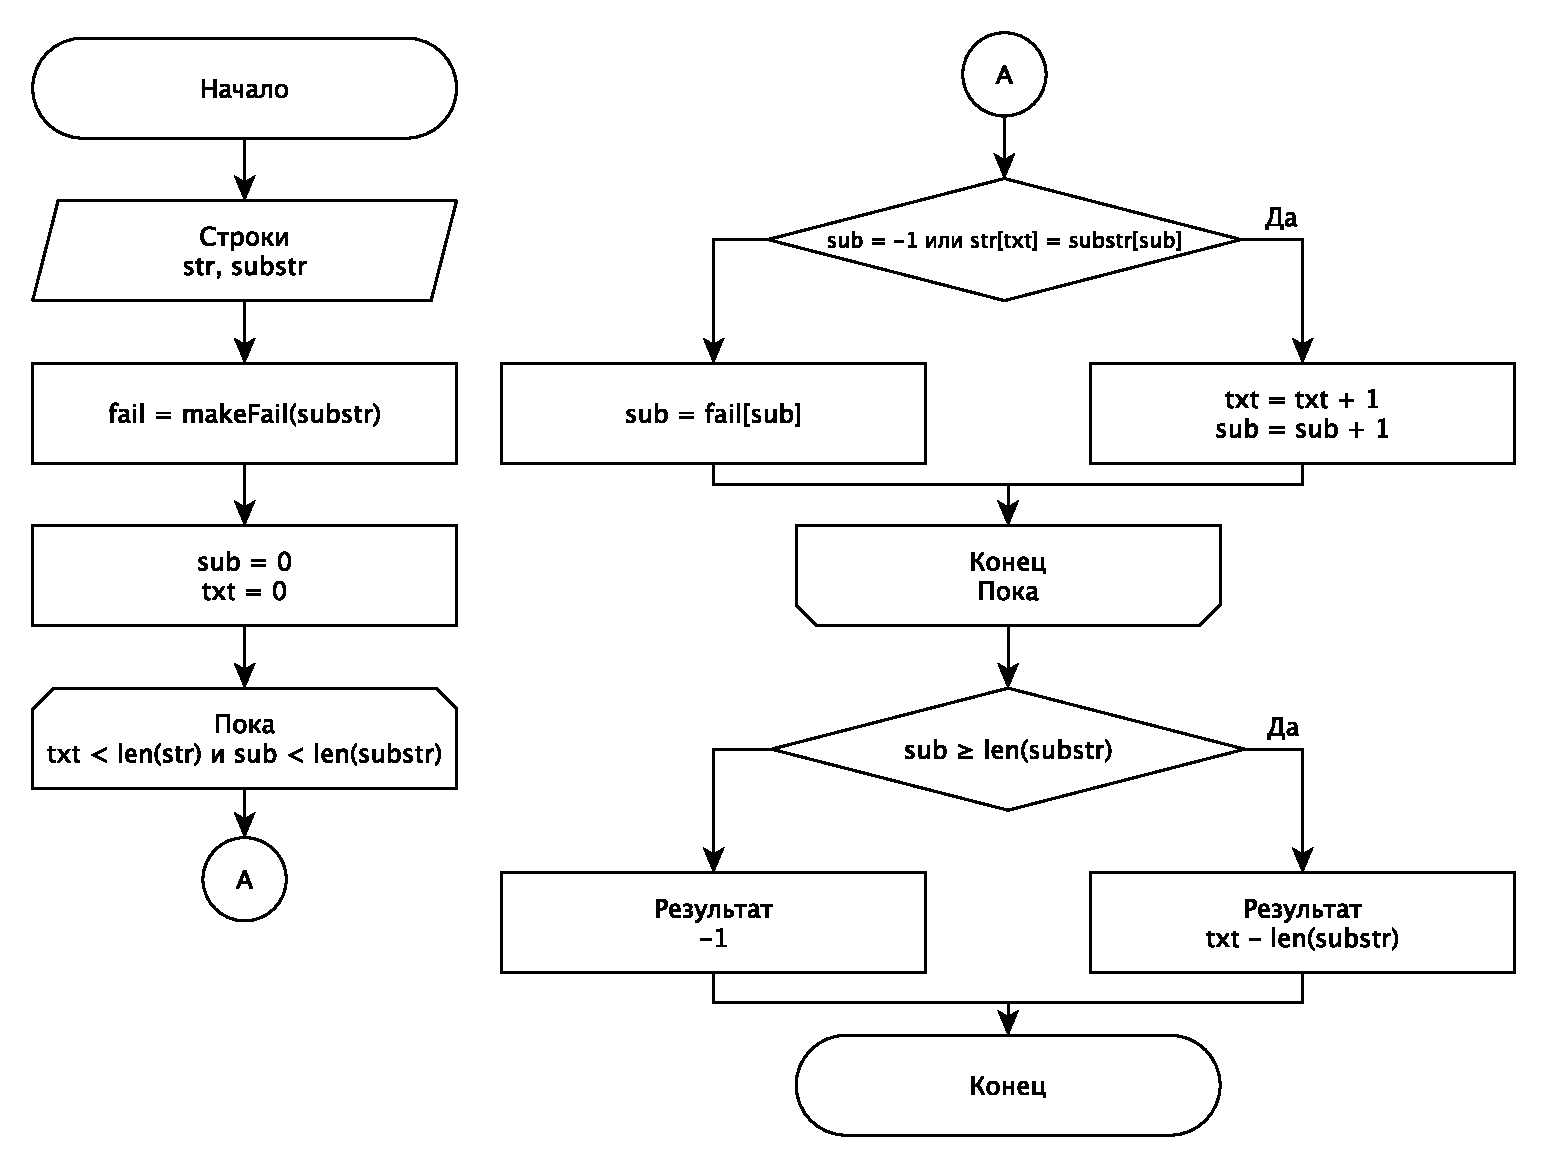
\includegraphics[scale=0.65]{knuth_morris_pratt}
    \caption{Схема алгоритма Кнута-Морриса-Пратта}
    \label{img:kmp}
\end{figure}

\begin{figure}[H]
    \centering
    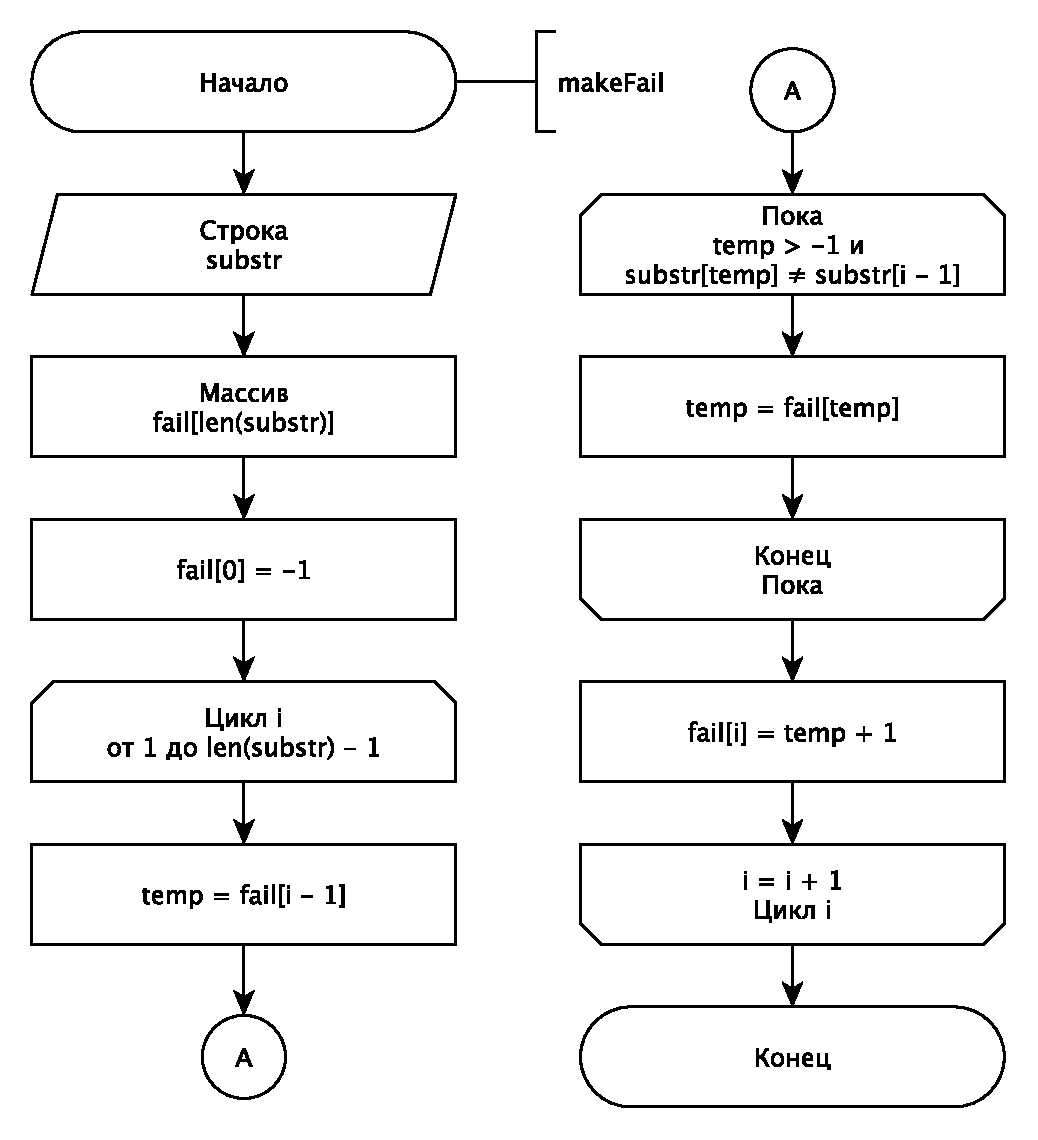
\includegraphics[scale=0.8]{fail}
    \caption{Схема алгоритма создания массива сдвигов}
    \label{img:fail}
\end{figure}

\begin{figure}[H]
    \centering
    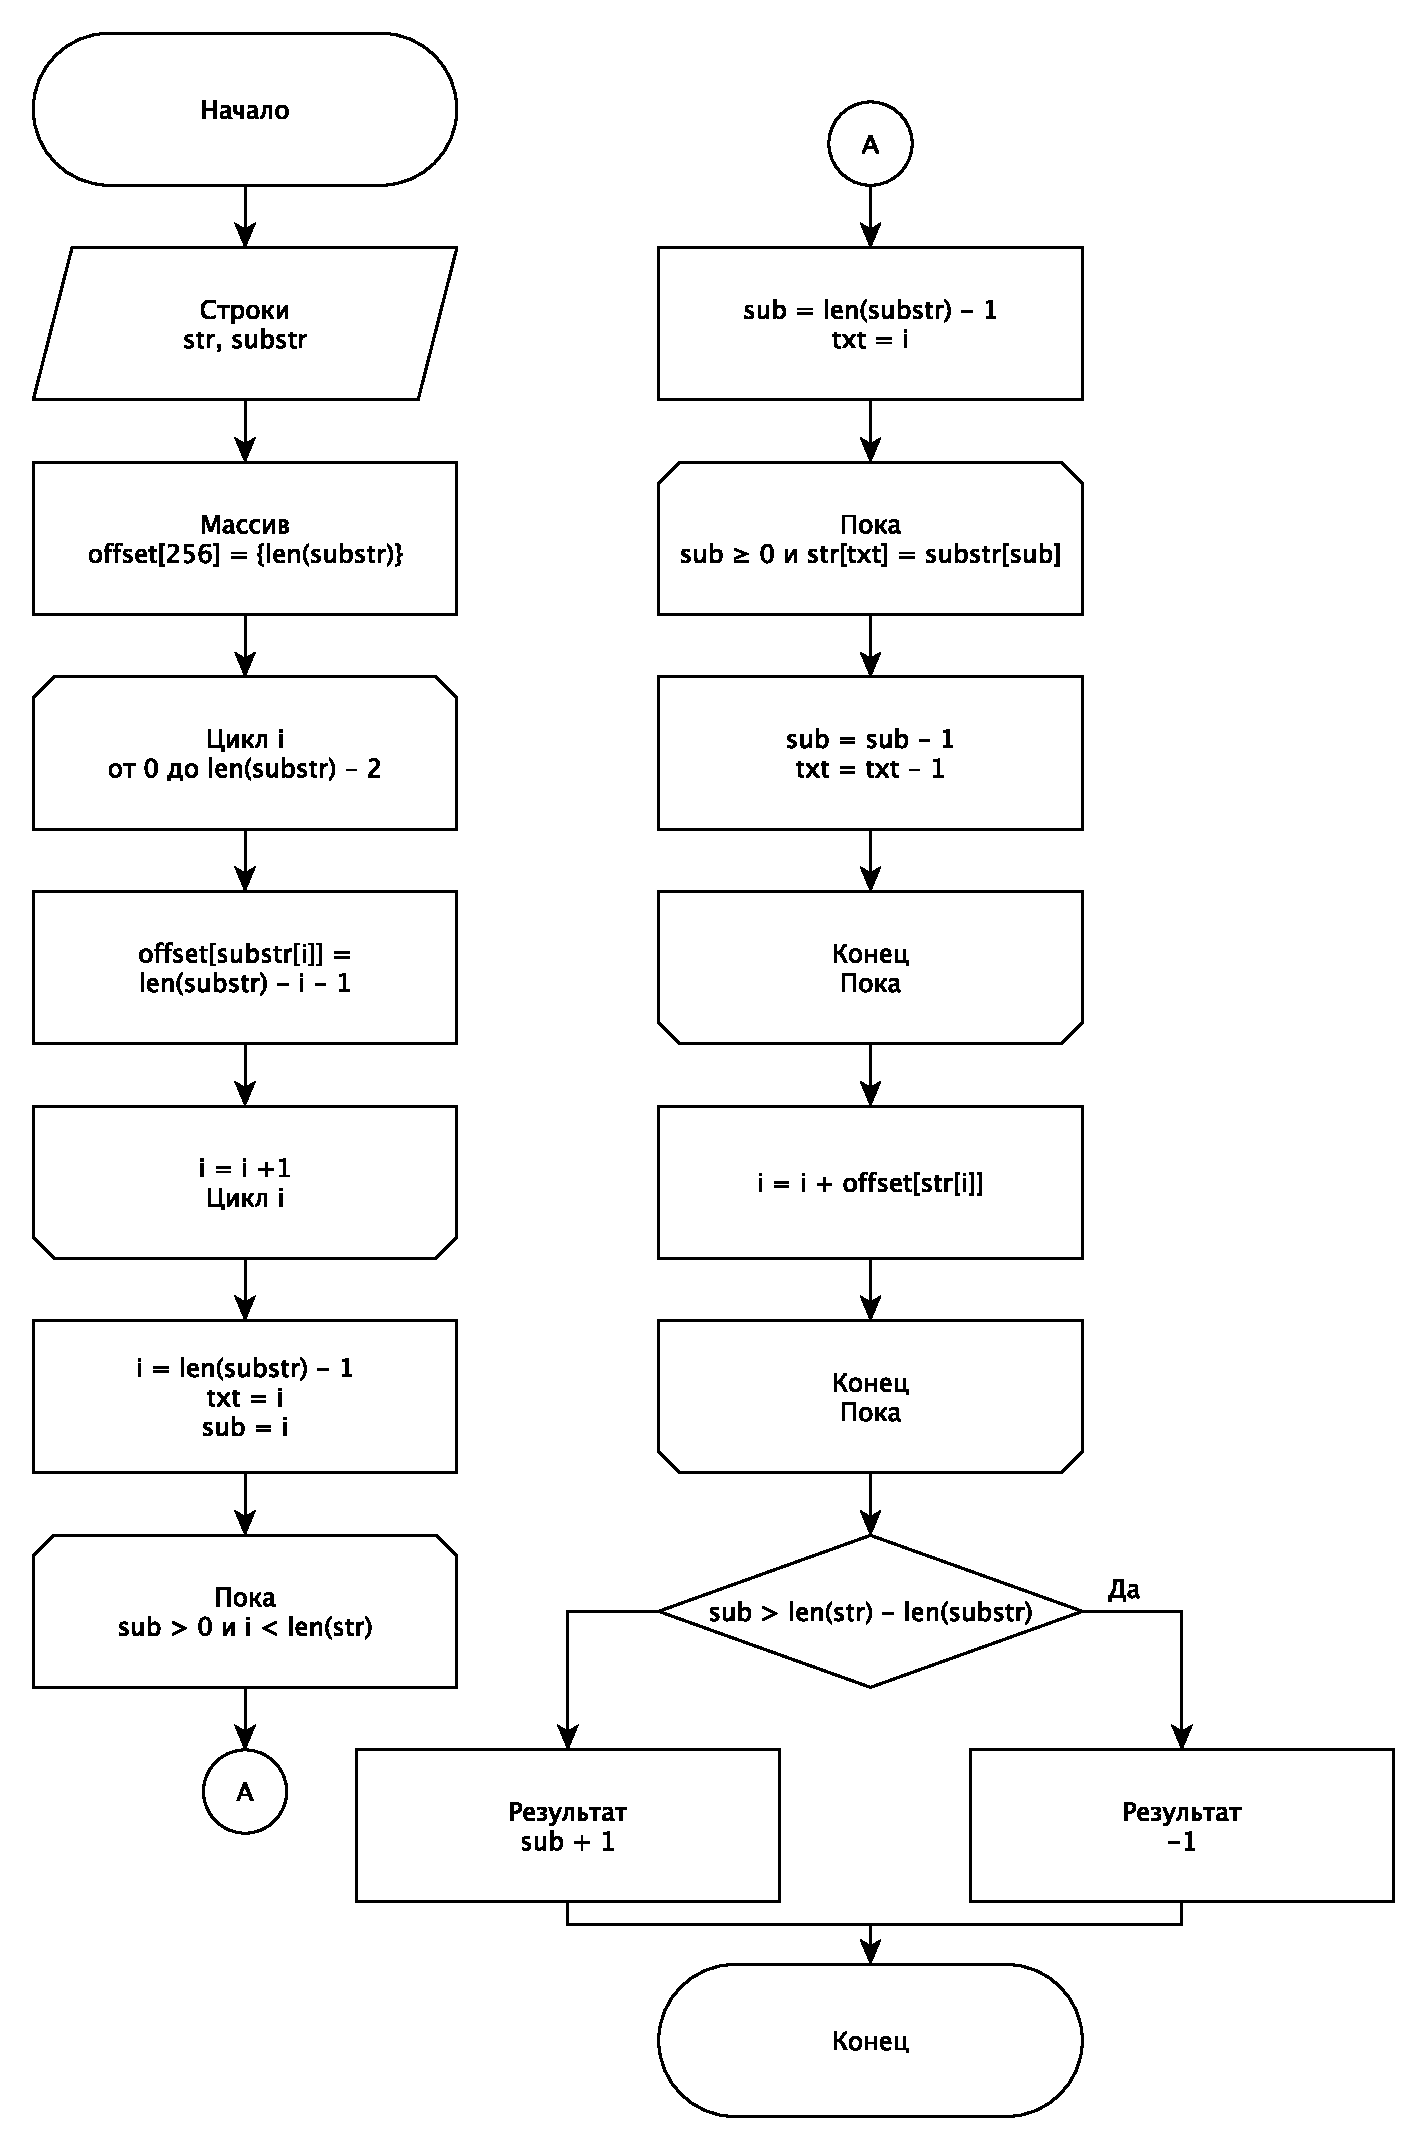
\includegraphics[scale=0.6]{boiler_myr}
    \caption{Схема алгоритма Бойлера-Мура}
    \label{img:bm}
\end{figure}

\subsection{Выводы}

Изучены алгоритмы поиска подстроки в строке, необходимо их реализовать.
